\documentclass[twoside]{book}

% Packages required by doxygen
\usepackage{fixltx2e}
\usepackage{calc}
\usepackage{doxygen}
\usepackage[export]{adjustbox} % also loads graphicx
\usepackage{graphicx}
\usepackage[utf8]{inputenc}
\usepackage{makeidx}
\usepackage{multicol}
\usepackage{multirow}
\PassOptionsToPackage{warn}{textcomp}
\usepackage{textcomp}
\usepackage[nointegrals]{wasysym}
\usepackage[table]{xcolor}

% Font selection
\usepackage[T1]{fontenc}
\usepackage[scaled=.90]{helvet}
\usepackage{courier}
\usepackage{amssymb}
\usepackage{sectsty}
\renewcommand{\familydefault}{\sfdefault}
\allsectionsfont{%
  \fontseries{bc}\selectfont%
  \color{darkgray}%
}
\renewcommand{\DoxyLabelFont}{%
  \fontseries{bc}\selectfont%
  \color{darkgray}%
}
\newcommand{\+}{\discretionary{\mbox{\scriptsize$\hookleftarrow$}}{}{}}

% Page & text layout
\usepackage{geometry}
\geometry{%
  a4paper,%
  top=2.5cm,%
  bottom=2.5cm,%
  left=2.5cm,%
  right=2.5cm%
}
\tolerance=750
\hfuzz=15pt
\hbadness=750
\setlength{\emergencystretch}{15pt}
\setlength{\parindent}{0cm}
\setlength{\parskip}{3ex plus 2ex minus 2ex}
\makeatletter
\renewcommand{\paragraph}{%
  \@startsection{paragraph}{4}{0ex}{-1.0ex}{1.0ex}{%
    \normalfont\normalsize\bfseries\SS@parafont%
  }%
}
\renewcommand{\subparagraph}{%
  \@startsection{subparagraph}{5}{0ex}{-1.0ex}{1.0ex}{%
    \normalfont\normalsize\bfseries\SS@subparafont%
  }%
}
\makeatother

% Headers & footers
\usepackage{fancyhdr}
\pagestyle{fancyplain}
\fancyhead[LE]{\fancyplain{}{\bfseries\thepage}}
\fancyhead[CE]{\fancyplain{}{}}
\fancyhead[RE]{\fancyplain{}{\bfseries\leftmark}}
\fancyhead[LO]{\fancyplain{}{\bfseries\rightmark}}
\fancyhead[CO]{\fancyplain{}{}}
\fancyhead[RO]{\fancyplain{}{\bfseries\thepage}}
\fancyfoot[LE]{\fancyplain{}{}}
\fancyfoot[CE]{\fancyplain{}{}}
\fancyfoot[RE]{\fancyplain{}{\bfseries\scriptsize Generated by Doxygen }}
\fancyfoot[LO]{\fancyplain{}{\bfseries\scriptsize Generated by Doxygen }}
\fancyfoot[CO]{\fancyplain{}{}}
\fancyfoot[RO]{\fancyplain{}{}}
\renewcommand{\footrulewidth}{0.4pt}
\renewcommand{\chaptermark}[1]{%
  \markboth{#1}{}%
}
\renewcommand{\sectionmark}[1]{%
  \markright{\thesection\ #1}%
}

% Indices & bibliography
\usepackage{natbib}
\usepackage[titles]{tocloft}
\setcounter{tocdepth}{3}
\setcounter{secnumdepth}{5}
\makeindex

% Hyperlinks (required, but should be loaded last)
\usepackage{ifpdf}
\ifpdf
  \usepackage[pdftex,pagebackref=true]{hyperref}
\else
  \usepackage[ps2pdf,pagebackref=true]{hyperref}
\fi
\hypersetup{%
  colorlinks=true,%
  linkcolor=blue,%
  citecolor=blue,%
  unicode%
}

% Custom commands
\newcommand{\clearemptydoublepage}{%
  \newpage{\pagestyle{empty}\cleardoublepage}%
}

\usepackage{caption}
\captionsetup{labelsep=space,justification=centering,font={bf},singlelinecheck=off,skip=4pt,position=top}

%===== C O N T E N T S =====

\begin{document}

% Titlepage & ToC
\hypersetup{pageanchor=false,
             bookmarksnumbered=true,
             pdfencoding=unicode
            }
\pagenumbering{alph}
\begin{titlepage}
\vspace*{7cm}
\begin{center}%
{\Large A\+UV Collision Detector }\\
\vspace*{1cm}
{\large Generated by Doxygen 1.8.13}\\
\end{center}
\end{titlepage}
\clearemptydoublepage
\pagenumbering{roman}
\tableofcontents
\clearemptydoublepage
\pagenumbering{arabic}
\hypersetup{pageanchor=true}

%--- Begin generated contents ---
\chapter{T\+O\+DO}
\label{md_README}
\Hypertarget{md_README}
\section*{D\+O\+C\+U\+M\+E\+N\+T\+A\+T\+I\+ON}

See the library documentation for further info \href{./html/index.html}{\tt } 
\chapter{Namespace Index}
\section{Namespace List}
Here is a list of all documented namespaces with brief descriptions\+:\begin{DoxyCompactList}
\item\contentsline{section}{\hyperlink{namespacecoldetector}{coldetector} \\*Namespace containing functions to perform the risk assessment process }{\pageref{namespacecoldetector}}{}
\end{DoxyCompactList}

\chapter{Class Index}
\section{Class List}
Here are the classes, structs, unions and interfaces with brief descriptions\+:\begin{DoxyCompactList}
\item\contentsline{section}{\hyperlink{classcoldetector_1_1CollisionDetector}{coldetector\+::\+Collision\+Detector} }{\pageref{classcoldetector_1_1CollisionDetector}}{}
\item\contentsline{section}{\hyperlink{classCollisionNode}{Collision\+Node} }{\pageref{classCollisionNode}}{}
\item\contentsline{section}{\hyperlink{classcSystem}{c\+System} }{\pageref{classcSystem}}{}
\item\contentsline{section}{\hyperlink{classMultiFrame}{Multi\+Frame} }{\pageref{classMultiFrame}}{}
\end{DoxyCompactList}

\chapter{Namespace Documentation}
\hypertarget{namespacecoldetector}{}\section{coldetector Namespace Reference}
\label{namespacecoldetector}\index{coldetector@{coldetector}}


Namespace containing functions to perform the risk assessment process.  


\subsection*{Classes}
\begin{DoxyCompactItemize}
\item 
class \hyperlink{classcoldetector_1_1CollisionDetector}{Collision\+Detector}
\end{DoxyCompactItemize}


\subsection{Detailed Description}
Namespace containing functions to perform the risk assessment process. 
\chapter{Class Documentation}
\hypertarget{classcoldetector_1_1CollisionDetector}{}\section{coldetector\+:\+:Collision\+Detector Class Reference}
\label{classcoldetector_1_1CollisionDetector}\index{coldetector\+::\+Collision\+Detector@{coldetector\+::\+Collision\+Detector}}


Collaboration diagram for coldetector\+:\+:Collision\+Detector\+:\nopagebreak
\begin{figure}[H]
\begin{center}
\leavevmode
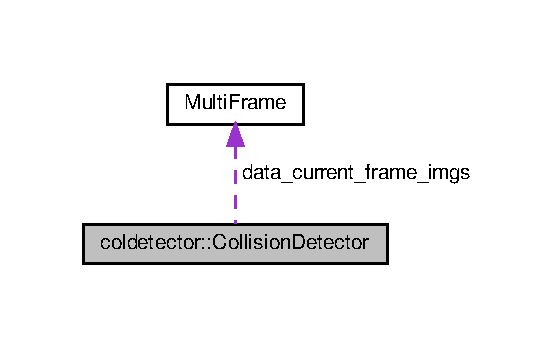
\includegraphics[width=267pt]{classcoldetector_1_1CollisionDetector__coll__graph}
\end{center}
\end{figure}
\subsection*{Public Member Functions}
\begin{DoxyCompactItemize}
\item 
\mbox{\Hypertarget{classcoldetector_1_1CollisionDetector_aa2169b92cec8e25c107622210b4c2872}\label{classcoldetector_1_1CollisionDetector_aa2169b92cec8e25c107622210b4c2872}} 
{\bfseries Collision\+Detector} (\hyperlink{classcSystem}{c\+System} $\ast$cam\+\_\+system, ros\+::\+Publisher $\ast$pc\+\_\+pub)
\item 
\mbox{\Hypertarget{classcoldetector_1_1CollisionDetector_af720f23bdcfe3536325fae4891d12ad8}\label{classcoldetector_1_1CollisionDetector_af720f23bdcfe3536325fae4891d12ad8}} 
void \hyperlink{classcoldetector_1_1CollisionDetector_af720f23bdcfe3536325fae4891d12ad8}{assign\+Chassis\+Points} ()
\begin{DoxyCompactList}\small\item\em Function that initialize a set of 3D points for the A\+UV chassis. These points are used later for assesing the risk. \end{DoxyCompactList}\item 
void \hyperlink{classcoldetector_1_1CollisionDetector_aa09c4115cdb0c5e3c0ecb3a29d3aac96}{Run} ()
\begin{DoxyCompactList}\small\item\em Obtains a pair of images and the estimated poses (v\+S\+L\+Am, I\+NS data) and processed them to obtain the 3D points of the robot surroundings. \end{DoxyCompactList}\item 
bool \hyperlink{classcoldetector_1_1CollisionDetector_aa4b6c5b052532e545758f84a668b43b2}{Check\+Data\+Availability} ()
\begin{DoxyCompactList}\small\item\em Checks if new image and pose data is available from the system and copies them for processing. \end{DoxyCompactList}\item 
void \hyperlink{classcoldetector_1_1CollisionDetector_a41e80df83d6f79de79798674bef21156}{transfer\+Data} (const \hyperlink{classMultiFrame}{Multi\+Frame} \&F, bool new\+\_\+data)
\begin{DoxyCompactList}\small\item\em Transfers data from the main program to the collision detection thread. \end{DoxyCompactList}\item 
void \hyperlink{classcoldetector_1_1CollisionDetector_a3e5a171f0d396656745e84b8e7a80cd9}{Frames\+Update} (\hyperlink{classMultiFrame}{Multi\+Frame} \&current\+\_\+frame)
\begin{DoxyCompactList}\small\item\em Updates the previous\+\_\+frame data with the current\+\_\+frame that was already processed. \end{DoxyCompactList}\item 
void \hyperlink{classcoldetector_1_1CollisionDetector_a01855b9eb3534d701df52f0f503fdc1e}{Get\+Relative\+Transformation\+Between\+Frames} (const cv\+::\+Mat \&base\+\_\+\+T\+\_\+cam, const cv\+::\+Mat \&world\+\_\+\+Tprevious\+\_\+base, const cv\+::\+Mat \&world\+\_\+\+Tcurrent\+\_\+base, cv\+::\+Mat \&cam\+\_\+previous\+\_\+\+T\+\_\+cam\+\_\+current)
\begin{DoxyCompactList}\small\item\em Computes the relative transformation between two frames. \end{DoxyCompactList}\item 
void \hyperlink{classcoldetector_1_1CollisionDetector_af385733b461bda4f537cb97f7616a352}{Compute\+Features} (const cv\+::\+Mat \&previous\+\_\+image\+\_\+cam\+\_\+i, const cv\+::\+Mat \&current\+\_\+image\+\_\+cam\+\_\+i, std\+::vector$<$ cv\+::\+Key\+Point $>$ \&keypoints\+\_\+previous\+\_\+i, std\+::vector$<$ cv\+::\+Key\+Point $>$ \&keypoints\+\_\+current\+\_\+i, cv\+::\+Mat \&descriptors\+\_\+previous\+\_\+i, cv\+::\+Mat \&descriptors\+\_\+current\+\_\+i)
\begin{DoxyCompactList}\small\item\em Compute keypoints and its descriptors in two images. \end{DoxyCompactList}\item 
void \hyperlink{classcoldetector_1_1CollisionDetector_ada1b7a3f4693f782da90feb111a59acc}{Compute\+Fundamental\+Matrix} (const cv\+::\+Mat \&current\+\_\+\+T\+\_\+previous, const cv\+::\+Mat cam\+\_\+K, cv\+::\+Mat \&current\+\_\+\+F\+\_\+previous)
\begin{DoxyCompactList}\small\item\em Compute the Fundamental matrix between two frames given their relative transformation matrix. \end{DoxyCompactList}\item 
void \hyperlink{classcoldetector_1_1CollisionDetector_a1cf35720359d0e9571e8ec233b6c2238}{Compute\+Matches\+Allvs\+All} (const cv\+::\+Mat \&descriptors\+\_\+previous\+\_\+i, const cv\+::\+Mat \&descriptors\+\_\+current\+\_\+i, std\+::vector$<$ cv\+::\+D\+Match $>$ \&best\+\_\+matches)
\begin{DoxyCompactList}\small\item\em Performs Brute force matching (all vs all) from a set of previous\+\_\+keypoints and current\+\_\+keypoints. \end{DoxyCompactList}\item 
void \hyperlink{classcoldetector_1_1CollisionDetector_a3464d9594b80dcda080bff19f7f9f9e3}{Filter\+Matches\+By\+Epipolar\+Constrain} (const std\+::vector$<$ cv\+::\+Key\+Point $>$ \&keypoints\+\_\+previous\+\_\+i, const std\+::vector$<$ cv\+::\+Key\+Point $>$ \&keypoints\+\_\+current\+\_\+i, const std\+::vector$<$ cv\+::\+D\+Match $>$ \&best\+\_\+matches, const cv\+::\+Mat \&F\+\_\+matrix, std\+::vector$<$ cv\+::\+D\+Match $>$ \&filtered\+\_\+matches)
\begin{DoxyCompactList}\small\item\em Uses epipolar geometry to filter the matches from a set of two images. \end{DoxyCompactList}\item 
void \hyperlink{classcoldetector_1_1CollisionDetector_a2027843784c5be77bebbad2785de51a7}{From\+Matches\+To\+Vectorof\+Points} (const std\+::vector$<$ cv\+::\+Key\+Point $>$ \&keypoints\+\_\+frame1, const std\+::vector$<$ cv\+::\+Key\+Point $>$ \&keypoints\+\_\+frame2, const std\+::vector$<$ cv\+::\+D\+Match $>$ \&matches, std\+::vector$<$ cv\+::\+Point2f $>$ \&points\+\_\+frame1, std\+::vector$<$ cv\+::\+Point2f $>$ \&points\+\_\+frame2)
\begin{DoxyCompactList}\small\item\em Transforms a vector of D\+Match type into a Point2d object. \end{DoxyCompactList}\item 
double \hyperlink{classcoldetector_1_1CollisionDetector_a27a359ba9c0c7b6966211ab35326179a}{Distance\+Point\+To\+Line} (const cv\+::\+Point2f point, const cv\+::\+Vec3f epiline)
\begin{DoxyCompactList}\small\item\em Computes the orthogonal distances from a 2D point to a line. \end{DoxyCompactList}\item 
void \hyperlink{classcoldetector_1_1CollisionDetector_a9b07097107a9acbf91bb5e338998d2c6}{Triangulate\+Points} (const cv\+::\+Mat \&base\+\_\+\+Tcam, const cv\+::\+Mat cam\+\_\+K, const cv\+::\+Mat \&current\+\_\+\+T\+\_\+previous, const std\+::vector$<$ cv\+::\+Key\+Point $>$ \&keypoints\+\_\+previous\+\_\+i, const std\+::vector$<$ cv\+::\+Key\+Point $>$ \&keypoints\+\_\+current\+\_\+i, const cv\+::\+Mat \&descriptors\+\_\+previous\+\_\+i, const cv\+::\+Mat \&descriptors\+\_\+current\+\_\+i, const std\+::vector$<$ cv\+::\+D\+Match $>$ \&filtered\+\_\+matches, const cv\+::\+Mat \&world\+\_\+\+Tcurrent\+\_\+base, bool b\+\_\+to\+\_\+world, std\+::vector$<$ cv\+::\+Mat $>$ \&final\+\_\+3d\+\_\+pts, cv\+::\+Mat \&final\+\_\+descriptors)
\begin{DoxyCompactList}\small\item\em Triangulate 3D points from a set of corresponding 2D matches. \end{DoxyCompactList}\item 
void \hyperlink{classcoldetector_1_1CollisionDetector_a432e4c735be67180cc599c2353e00beb}{Compute\+Projection\+Matrices} (const cv\+::\+Mat cam\+\_\+K, const cv\+::\+Mat \&current\+\_\+\+T\+\_\+previous, cv\+::\+Mat \&P\+\_\+previous, cv\+::\+Mat \&P\+\_\+current)
\begin{DoxyCompactList}\small\item\em Computes the Projection matrices of two frames. \end{DoxyCompactList}\item 
void \hyperlink{classcoldetector_1_1CollisionDetector_abf7f01bfb82b58af9683d565a901659d}{Get\+Array\+Of\+Points} (std\+::vector$<$ cv\+::\+Point2f $>$ \&points\+\_\+frame1, std\+::vector$<$ cv\+::\+Point2f $>$ \&points\+\_\+frame2, std\+::vector$<$ cv\+::\+Mat $>$ \&array\+\_\+of\+\_\+points)
\begin{DoxyCompactList}\small\item\em Adjust a set of cv\+:Point2f vector arrays into an Input\+Array\+Of\+Arrays object. \end{DoxyCompactList}\item 
\mbox{\Hypertarget{classcoldetector_1_1CollisionDetector_a94abb97b8bce8c4c839ba36696667adc}\label{classcoldetector_1_1CollisionDetector_a94abb97b8bce8c4c839ba36696667adc}} 
void \hyperlink{classcoldetector_1_1CollisionDetector_a94abb97b8bce8c4c839ba36696667adc}{Stop\+Request} ()
\begin{DoxyCompactList}\small\item\em Stops the thread when requested from the main program. \end{DoxyCompactList}\end{DoxyCompactItemize}
\subsection*{Public Attributes}
\begin{DoxyCompactItemize}
\item 
\mbox{\Hypertarget{classcoldetector_1_1CollisionDetector_a6fa9191f807302da1bb1fae0d006be16}\label{classcoldetector_1_1CollisionDetector_a6fa9191f807302da1bb1fae0d006be16}} 
bool {\bfseries b\+\_\+do\+\_\+clahe\+\_\+}
\item 
\mbox{\Hypertarget{classcoldetector_1_1CollisionDetector_a8db158921586ac5eac43de655d2a49bf}\label{classcoldetector_1_1CollisionDetector_a8db158921586ac5eac43de655d2a49bf}} 
bool {\bfseries b\+\_\+matching\+\_\+all\+\_\+all\+\_\+}
\item 
\mbox{\Hypertarget{classcoldetector_1_1CollisionDetector_a876a4626ad6f0b42eca1015736c08b12}\label{classcoldetector_1_1CollisionDetector_a876a4626ad6f0b42eca1015736c08b12}} 
bool {\bfseries b\+\_\+pointcloud\+\_\+in\+\_\+world\+\_\+}
\item 
\mbox{\Hypertarget{classcoldetector_1_1CollisionDetector_ab456210400a1ba6ef873609dcf8317ee}\label{classcoldetector_1_1CollisionDetector_ab456210400a1ba6ef873609dcf8317ee}} 
bool {\bfseries b\+\_\+consider\+\_\+chassis\+\_\+b\+\_\+}
\item 
\mbox{\Hypertarget{classcoldetector_1_1CollisionDetector_ab23340a36c5a6de7ad9f57acfc2f07de}\label{classcoldetector_1_1CollisionDetector_ab23340a36c5a6de7ad9f57acfc2f07de}} 
bool {\bfseries b\+\_\+new\+\_\+data\+\_\+}
\item 
\mbox{\Hypertarget{classcoldetector_1_1CollisionDetector_ad71e38040d7e6f64ee79d095915321fe}\label{classcoldetector_1_1CollisionDetector_ad71e38040d7e6f64ee79d095915321fe}} 
\hyperlink{classMultiFrame}{Multi\+Frame} {\bfseries data\+\_\+current\+\_\+frame\+\_\+imgs}
\item 
\mbox{\Hypertarget{classcoldetector_1_1CollisionDetector_acda0507fbb212fe54a1165bd2b388c6d}\label{classcoldetector_1_1CollisionDetector_acda0507fbb212fe54a1165bd2b388c6d}} 
cv\+::\+Matx$<$ double, 4, 4 $>$ {\bfseries data\+\_\+current\+\_\+pose}
\item 
\mbox{\Hypertarget{classcoldetector_1_1CollisionDetector_a3f9726dab2adda41e3c9a20dd496e0bd}\label{classcoldetector_1_1CollisionDetector_a3f9726dab2adda41e3c9a20dd496e0bd}} 
std\+::mutex {\bfseries m\+Receive\+Data}
\item 
\mbox{\Hypertarget{classcoldetector_1_1CollisionDetector_a7d4d389640ecf22e2c8d3bed14d187fb}\label{classcoldetector_1_1CollisionDetector_a7d4d389640ecf22e2c8d3bed14d187fb}} 
std\+::mutex {\bfseries m\+Mutex\+Stop}
\end{DoxyCompactItemize}


\subsection{Member Function Documentation}
\mbox{\Hypertarget{classcoldetector_1_1CollisionDetector_aa4b6c5b052532e545758f84a668b43b2}\label{classcoldetector_1_1CollisionDetector_aa4b6c5b052532e545758f84a668b43b2}} 
\index{coldetector\+::\+Collision\+Detector@{coldetector\+::\+Collision\+Detector}!Check\+Data\+Availability@{Check\+Data\+Availability}}
\index{Check\+Data\+Availability@{Check\+Data\+Availability}!coldetector\+::\+Collision\+Detector@{coldetector\+::\+Collision\+Detector}}
\subsubsection{\texorpdfstring{Check\+Data\+Availability()}{CheckDataAvailability()}}
{\footnotesize\ttfamily bool coldetector\+::\+Collision\+Detector\+::\+Check\+Data\+Availability (\begin{DoxyParamCaption}{ }\end{DoxyParamCaption})}



Checks if new image and pose data is available from the system and copies them for processing. 

\begin{DoxyReturn}{Returns}
temp Flag that indicates wether if new data has been receieved or not. 
\end{DoxyReturn}
\mbox{\Hypertarget{classcoldetector_1_1CollisionDetector_af385733b461bda4f537cb97f7616a352}\label{classcoldetector_1_1CollisionDetector_af385733b461bda4f537cb97f7616a352}} 
\index{coldetector\+::\+Collision\+Detector@{coldetector\+::\+Collision\+Detector}!Compute\+Features@{Compute\+Features}}
\index{Compute\+Features@{Compute\+Features}!coldetector\+::\+Collision\+Detector@{coldetector\+::\+Collision\+Detector}}
\subsubsection{\texorpdfstring{Compute\+Features()}{ComputeFeatures()}}
{\footnotesize\ttfamily void coldetector\+::\+Collision\+Detector\+::\+Compute\+Features (\begin{DoxyParamCaption}\item[{const cv\+::\+Mat \&}]{previous\+\_\+image\+\_\+cam\+\_\+i,  }\item[{const cv\+::\+Mat \&}]{current\+\_\+image\+\_\+cam\+\_\+i,  }\item[{std\+::vector$<$ cv\+::\+Key\+Point $>$ \&}]{keypoints\+\_\+previous\+\_\+i,  }\item[{std\+::vector$<$ cv\+::\+Key\+Point $>$ \&}]{keypoints\+\_\+current\+\_\+i,  }\item[{cv\+::\+Mat \&}]{descriptors\+\_\+previous\+\_\+i,  }\item[{cv\+::\+Mat \&}]{descriptors\+\_\+current\+\_\+i }\end{DoxyParamCaption})}



Compute keypoints and its descriptors in two images. 


\begin{DoxyParams}{Parameters}
{\em previous\+\_\+image\+\_\+cam\+\_\+i} & Image of camera i in the previous frame. \\
\hline
{\em current\+\_\+image\+\_\+cam\+\_\+i} & Image of camera i in the currnet frame. \\
\hline
{\em keypoints\+\_\+previous\+\_\+i} & Output vector of cv\+::\+Keypoints corresponding to features detected on previous frame. \\
\hline
{\em keypoints\+\_\+current\+\_\+i} & Output vector of cv\+::\+Keypoints corresponding to features detected on current frame. \\
\hline
{\em descriptors\+\_\+previous\+\_\+i} & Output vector of corresponding descriptors on previous frame. \\
\hline
{\em descriptors\+\_\+current\+\_\+i} & Output vector of corresponding descriptors on current frame. \\
\hline
\end{DoxyParams}
\mbox{\Hypertarget{classcoldetector_1_1CollisionDetector_ada1b7a3f4693f782da90feb111a59acc}\label{classcoldetector_1_1CollisionDetector_ada1b7a3f4693f782da90feb111a59acc}} 
\index{coldetector\+::\+Collision\+Detector@{coldetector\+::\+Collision\+Detector}!Compute\+Fundamental\+Matrix@{Compute\+Fundamental\+Matrix}}
\index{Compute\+Fundamental\+Matrix@{Compute\+Fundamental\+Matrix}!coldetector\+::\+Collision\+Detector@{coldetector\+::\+Collision\+Detector}}
\subsubsection{\texorpdfstring{Compute\+Fundamental\+Matrix()}{ComputeFundamentalMatrix()}}
{\footnotesize\ttfamily void coldetector\+::\+Collision\+Detector\+::\+Compute\+Fundamental\+Matrix (\begin{DoxyParamCaption}\item[{const cv\+::\+Mat \&}]{current\+\_\+\+T\+\_\+previous,  }\item[{const cv\+::\+Mat}]{cam\+\_\+K,  }\item[{cv\+::\+Mat \&}]{current\+\_\+\+F\+\_\+previous }\end{DoxyParamCaption})}



Compute the Fundamental matrix between two frames given their relative transformation matrix. 


\begin{DoxyParams}{Parameters}
{\em current\+\_\+\+T\+\_\+previous} & relative transformation matrix of previous frame w.\+r.\+t the current frame. \\
\hline
{\em cam\+\_\+K} & The instrinsic parameters of the camera. \\
\hline
{\em current\+\_\+\+F\+\_\+previous} & Output Fundamental matrix of the previous frame w.\+r.\+t. the current frame. \\
\hline
\end{DoxyParams}
\mbox{\Hypertarget{classcoldetector_1_1CollisionDetector_a1cf35720359d0e9571e8ec233b6c2238}\label{classcoldetector_1_1CollisionDetector_a1cf35720359d0e9571e8ec233b6c2238}} 
\index{coldetector\+::\+Collision\+Detector@{coldetector\+::\+Collision\+Detector}!Compute\+Matches\+Allvs\+All@{Compute\+Matches\+Allvs\+All}}
\index{Compute\+Matches\+Allvs\+All@{Compute\+Matches\+Allvs\+All}!coldetector\+::\+Collision\+Detector@{coldetector\+::\+Collision\+Detector}}
\subsubsection{\texorpdfstring{Compute\+Matches\+Allvs\+All()}{ComputeMatchesAllvsAll()}}
{\footnotesize\ttfamily void coldetector\+::\+Collision\+Detector\+::\+Compute\+Matches\+Allvs\+All (\begin{DoxyParamCaption}\item[{const cv\+::\+Mat \&}]{descriptors\+\_\+previous\+\_\+i,  }\item[{const cv\+::\+Mat \&}]{descriptors\+\_\+current\+\_\+i,  }\item[{std\+::vector$<$ cv\+::\+D\+Match $>$ \&}]{best\+\_\+matches }\end{DoxyParamCaption})}



Performs Brute force matching (all vs all) from a set of previous\+\_\+keypoints and current\+\_\+keypoints. 


\begin{DoxyParams}{Parameters}
{\em descriptors\+\_\+previous\+\_\+i} & Descriptors computed on the previous frame. \\
\hline
{\em descriptors\+\_\+current\+\_\+i} & Descriptors computed on the current frame. \\
\hline
{\em best\+\_\+matches} & Output vector with matches that satisfy the Lowe\textquotesingle{}s ratio test. \\
\hline
\end{DoxyParams}
\mbox{\Hypertarget{classcoldetector_1_1CollisionDetector_a432e4c735be67180cc599c2353e00beb}\label{classcoldetector_1_1CollisionDetector_a432e4c735be67180cc599c2353e00beb}} 
\index{coldetector\+::\+Collision\+Detector@{coldetector\+::\+Collision\+Detector}!Compute\+Projection\+Matrices@{Compute\+Projection\+Matrices}}
\index{Compute\+Projection\+Matrices@{Compute\+Projection\+Matrices}!coldetector\+::\+Collision\+Detector@{coldetector\+::\+Collision\+Detector}}
\subsubsection{\texorpdfstring{Compute\+Projection\+Matrices()}{ComputeProjectionMatrices()}}
{\footnotesize\ttfamily void coldetector\+::\+Collision\+Detector\+::\+Compute\+Projection\+Matrices (\begin{DoxyParamCaption}\item[{const cv\+::\+Mat}]{cam\+\_\+K,  }\item[{const cv\+::\+Mat \&}]{current\+\_\+\+T\+\_\+previous,  }\item[{cv\+::\+Mat \&}]{P\+\_\+previous,  }\item[{cv\+::\+Mat \&}]{P\+\_\+current }\end{DoxyParamCaption})}



Computes the Projection matrices of two frames. 


\begin{DoxyParams}{Parameters}
{\em cam\+\_\+K} & The instrinsic parameters of the camera. \\
\hline
{\em current\+\_\+\+T\+\_\+previous} & The relative transformation of image 2 w.\+r.\+t image 1. \\
\hline
{\em P\+\_\+previous} & Output Projection matrix of the previous frame. \\
\hline
{\em P\+\_\+current} & Output Projection matrix of the current frame. \\
\hline
\end{DoxyParams}
\mbox{\Hypertarget{classcoldetector_1_1CollisionDetector_a27a359ba9c0c7b6966211ab35326179a}\label{classcoldetector_1_1CollisionDetector_a27a359ba9c0c7b6966211ab35326179a}} 
\index{coldetector\+::\+Collision\+Detector@{coldetector\+::\+Collision\+Detector}!Distance\+Point\+To\+Line@{Distance\+Point\+To\+Line}}
\index{Distance\+Point\+To\+Line@{Distance\+Point\+To\+Line}!coldetector\+::\+Collision\+Detector@{coldetector\+::\+Collision\+Detector}}
\subsubsection{\texorpdfstring{Distance\+Point\+To\+Line()}{DistancePointToLine()}}
{\footnotesize\ttfamily double coldetector\+::\+Collision\+Detector\+::\+Distance\+Point\+To\+Line (\begin{DoxyParamCaption}\item[{const cv\+::\+Point2f}]{point,  }\item[{const cv\+::\+Vec3f}]{epiline }\end{DoxyParamCaption})}



Computes the orthogonal distances from a 2D point to a line. 


\begin{DoxyParams}{Parameters}
{\em point} & The 2D point in the image. \\
\hline
{\em epiline} & The corresponding epipolar line. \\
\hline
\end{DoxyParams}
\begin{DoxyReturn}{Returns}
distance The orthogonal distance from the point to the line. 
\end{DoxyReturn}
\mbox{\Hypertarget{classcoldetector_1_1CollisionDetector_a3464d9594b80dcda080bff19f7f9f9e3}\label{classcoldetector_1_1CollisionDetector_a3464d9594b80dcda080bff19f7f9f9e3}} 
\index{coldetector\+::\+Collision\+Detector@{coldetector\+::\+Collision\+Detector}!Filter\+Matches\+By\+Epipolar\+Constrain@{Filter\+Matches\+By\+Epipolar\+Constrain}}
\index{Filter\+Matches\+By\+Epipolar\+Constrain@{Filter\+Matches\+By\+Epipolar\+Constrain}!coldetector\+::\+Collision\+Detector@{coldetector\+::\+Collision\+Detector}}
\subsubsection{\texorpdfstring{Filter\+Matches\+By\+Epipolar\+Constrain()}{FilterMatchesByEpipolarConstrain()}}
{\footnotesize\ttfamily void coldetector\+::\+Collision\+Detector\+::\+Filter\+Matches\+By\+Epipolar\+Constrain (\begin{DoxyParamCaption}\item[{const std\+::vector$<$ cv\+::\+Key\+Point $>$ \&}]{keypoints\+\_\+previous\+\_\+i,  }\item[{const std\+::vector$<$ cv\+::\+Key\+Point $>$ \&}]{keypoints\+\_\+current\+\_\+i,  }\item[{const std\+::vector$<$ cv\+::\+D\+Match $>$ \&}]{best\+\_\+matches,  }\item[{const cv\+::\+Mat \&}]{F\+\_\+matrix,  }\item[{std\+::vector$<$ cv\+::\+D\+Match $>$ \&}]{filtered\+\_\+matches }\end{DoxyParamCaption})}



Uses epipolar geometry to filter the matches from a set of two images. 


\begin{DoxyParams}{Parameters}
{\em keypoints\+\_\+previous\+\_\+i} & Features detected on previous frame. \\
\hline
{\em keypoints\+\_\+current\+\_\+i} & Features detected on current frame. \\
\hline
{\em best\+\_\+matches} & Set of feature matches between images. \\
\hline
{\em F\+\_\+matrix} & Fundamental matrix of the previous frame w.\+r.\+t. the current frame. \\
\hline
{\em filtered\+\_\+matches} & Output vector with all the feature matches that satisfy the epipolar constraint. \\
\hline
\end{DoxyParams}
\mbox{\Hypertarget{classcoldetector_1_1CollisionDetector_a3e5a171f0d396656745e84b8e7a80cd9}\label{classcoldetector_1_1CollisionDetector_a3e5a171f0d396656745e84b8e7a80cd9}} 
\index{coldetector\+::\+Collision\+Detector@{coldetector\+::\+Collision\+Detector}!Frames\+Update@{Frames\+Update}}
\index{Frames\+Update@{Frames\+Update}!coldetector\+::\+Collision\+Detector@{coldetector\+::\+Collision\+Detector}}
\subsubsection{\texorpdfstring{Frames\+Update()}{FramesUpdate()}}
{\footnotesize\ttfamily void coldetector\+::\+Collision\+Detector\+::\+Frames\+Update (\begin{DoxyParamCaption}\item[{\hyperlink{classMultiFrame}{Multi\+Frame} \&}]{current\+\_\+frame }\end{DoxyParamCaption})}



Updates the previous\+\_\+frame data with the current\+\_\+frame that was already processed. 


\begin{DoxyParams}{Parameters}
{\em current\+\_\+frame} & Frame data corresponding to the newly processed data. \\
\hline
\end{DoxyParams}
\mbox{\Hypertarget{classcoldetector_1_1CollisionDetector_a2027843784c5be77bebbad2785de51a7}\label{classcoldetector_1_1CollisionDetector_a2027843784c5be77bebbad2785de51a7}} 
\index{coldetector\+::\+Collision\+Detector@{coldetector\+::\+Collision\+Detector}!From\+Matches\+To\+Vectorof\+Points@{From\+Matches\+To\+Vectorof\+Points}}
\index{From\+Matches\+To\+Vectorof\+Points@{From\+Matches\+To\+Vectorof\+Points}!coldetector\+::\+Collision\+Detector@{coldetector\+::\+Collision\+Detector}}
\subsubsection{\texorpdfstring{From\+Matches\+To\+Vectorof\+Points()}{FromMatchesToVectorofPoints()}}
{\footnotesize\ttfamily void coldetector\+::\+Collision\+Detector\+::\+From\+Matches\+To\+Vectorof\+Points (\begin{DoxyParamCaption}\item[{const std\+::vector$<$ cv\+::\+Key\+Point $>$ \&}]{keypoints\+\_\+frame1,  }\item[{const std\+::vector$<$ cv\+::\+Key\+Point $>$ \&}]{keypoints\+\_\+frame2,  }\item[{const std\+::vector$<$ cv\+::\+D\+Match $>$ \&}]{matches,  }\item[{std\+::vector$<$ cv\+::\+Point2f $>$ \&}]{points\+\_\+frame1,  }\item[{std\+::vector$<$ cv\+::\+Point2f $>$ \&}]{points\+\_\+frame2 }\end{DoxyParamCaption})}



Transforms a vector of D\+Match type into a Point2d object. 


\begin{DoxyParams}{Parameters}
{\em keypoints\+\_\+frame1} & Features detected on frame 1. \\
\hline
{\em keypoints\+\_\+frame2} & Features detected on frame 2. \\
\hline
{\em matches} & Vector of the computed matches between frames. \\
\hline
{\em points\+\_\+frame1} & Output vector of cv\+::\+Point2f 2D points on frame 1. \\
\hline
{\em points\+\_\+frame2} & Output vector of cv\+::\+Point2f 2D points on frame 2. \\
\hline
\end{DoxyParams}
\mbox{\Hypertarget{classcoldetector_1_1CollisionDetector_abf7f01bfb82b58af9683d565a901659d}\label{classcoldetector_1_1CollisionDetector_abf7f01bfb82b58af9683d565a901659d}} 
\index{coldetector\+::\+Collision\+Detector@{coldetector\+::\+Collision\+Detector}!Get\+Array\+Of\+Points@{Get\+Array\+Of\+Points}}
\index{Get\+Array\+Of\+Points@{Get\+Array\+Of\+Points}!coldetector\+::\+Collision\+Detector@{coldetector\+::\+Collision\+Detector}}
\subsubsection{\texorpdfstring{Get\+Array\+Of\+Points()}{GetArrayOfPoints()}}
{\footnotesize\ttfamily void coldetector\+::\+Collision\+Detector\+::\+Get\+Array\+Of\+Points (\begin{DoxyParamCaption}\item[{std\+::vector$<$ cv\+::\+Point2f $>$ \&}]{points\+\_\+frame1,  }\item[{std\+::vector$<$ cv\+::\+Point2f $>$ \&}]{points\+\_\+frame2,  }\item[{std\+::vector$<$ cv\+::\+Mat $>$ \&}]{array\+\_\+of\+\_\+points }\end{DoxyParamCaption})}



Adjust a set of cv\+:Point2f vector arrays into an Input\+Array\+Of\+Arrays object. 


\begin{DoxyParams}{Parameters}
{\em points\+\_\+frame1} & of cv\+::\+Point2f 2D points on frame 1. \\
\hline
{\em points\+\_\+frame2} & of cv\+::\+Point2f 2D points on frame 2. \\
\hline
{\em array\+\_\+of\+\_\+points} & Set of points converted to an std\+::vector of cv\+::\+Mat. \\
\hline
\end{DoxyParams}
\mbox{\Hypertarget{classcoldetector_1_1CollisionDetector_a01855b9eb3534d701df52f0f503fdc1e}\label{classcoldetector_1_1CollisionDetector_a01855b9eb3534d701df52f0f503fdc1e}} 
\index{coldetector\+::\+Collision\+Detector@{coldetector\+::\+Collision\+Detector}!Get\+Relative\+Transformation\+Between\+Frames@{Get\+Relative\+Transformation\+Between\+Frames}}
\index{Get\+Relative\+Transformation\+Between\+Frames@{Get\+Relative\+Transformation\+Between\+Frames}!coldetector\+::\+Collision\+Detector@{coldetector\+::\+Collision\+Detector}}
\subsubsection{\texorpdfstring{Get\+Relative\+Transformation\+Between\+Frames()}{GetRelativeTransformationBetweenFrames()}}
{\footnotesize\ttfamily void coldetector\+::\+Collision\+Detector\+::\+Get\+Relative\+Transformation\+Between\+Frames (\begin{DoxyParamCaption}\item[{const cv\+::\+Mat \&}]{base\+\_\+\+T\+\_\+cam,  }\item[{const cv\+::\+Mat \&}]{world\+\_\+\+Tprevious\+\_\+base,  }\item[{const cv\+::\+Mat \&}]{world\+\_\+\+Tcurrent\+\_\+base,  }\item[{cv\+::\+Mat \&}]{cam\+\_\+previous\+\_\+\+T\+\_\+cam\+\_\+current }\end{DoxyParamCaption})}



Computes the relative transformation between two frames. 


\begin{DoxyParams}{Parameters}
{\em base\+\_\+\+T\+\_\+cam} & Transformation of the camera i w.\+r.\+t to the camera origin. \\
\hline
{\em world\+\_\+\+Tprevious\+\_\+base} & Transformation of the camera origin w.\+r.\+t the world on the previous frame. \\
\hline
{\em world\+\_\+\+Tcurrent\+\_\+base} & Transformation of the camera origin w.\+r.\+t the world on the current frame. \\
\hline
{\em cam\+\_\+previous\+\_\+\+T\+\_\+cam\+\_\+current} & Output relative transformation matrix. \\
\hline
\end{DoxyParams}
\mbox{\Hypertarget{classcoldetector_1_1CollisionDetector_aa09c4115cdb0c5e3c0ecb3a29d3aac96}\label{classcoldetector_1_1CollisionDetector_aa09c4115cdb0c5e3c0ecb3a29d3aac96}} 
\index{coldetector\+::\+Collision\+Detector@{coldetector\+::\+Collision\+Detector}!Run@{Run}}
\index{Run@{Run}!coldetector\+::\+Collision\+Detector@{coldetector\+::\+Collision\+Detector}}
\subsubsection{\texorpdfstring{Run()}{Run()}}
{\footnotesize\ttfamily void coldetector\+::\+Collision\+Detector\+::\+Run (\begin{DoxyParamCaption}{ }\end{DoxyParamCaption})}



Obtains a pair of images and the estimated poses (v\+S\+L\+Am, I\+NS data) and processed them to obtain the 3D points of the robot surroundings. 

Get camera base poses w.\+r.\+t. the world

Process camera data \mbox{\Hypertarget{classcoldetector_1_1CollisionDetector_a41e80df83d6f79de79798674bef21156}\label{classcoldetector_1_1CollisionDetector_a41e80df83d6f79de79798674bef21156}} 
\index{coldetector\+::\+Collision\+Detector@{coldetector\+::\+Collision\+Detector}!transfer\+Data@{transfer\+Data}}
\index{transfer\+Data@{transfer\+Data}!coldetector\+::\+Collision\+Detector@{coldetector\+::\+Collision\+Detector}}
\subsubsection{\texorpdfstring{transfer\+Data()}{transferData()}}
{\footnotesize\ttfamily void coldetector\+::\+Collision\+Detector\+::transfer\+Data (\begin{DoxyParamCaption}\item[{const \hyperlink{classMultiFrame}{Multi\+Frame} \&}]{F,  }\item[{bool}]{new\+\_\+data }\end{DoxyParamCaption})}



Transfers data from the main program to the collision detection thread. 


\begin{DoxyParams}{Parameters}
{\em F} & \hyperlink{classMultiFrame}{Multi\+Frame} object that contains an array of N images, corresponding to each camera. \\
\hline
{\em new\+\_\+data} & Flag that indicates that new data has been received. \\
\hline
\end{DoxyParams}
\mbox{\Hypertarget{classcoldetector_1_1CollisionDetector_a9b07097107a9acbf91bb5e338998d2c6}\label{classcoldetector_1_1CollisionDetector_a9b07097107a9acbf91bb5e338998d2c6}} 
\index{coldetector\+::\+Collision\+Detector@{coldetector\+::\+Collision\+Detector}!Triangulate\+Points@{Triangulate\+Points}}
\index{Triangulate\+Points@{Triangulate\+Points}!coldetector\+::\+Collision\+Detector@{coldetector\+::\+Collision\+Detector}}
\subsubsection{\texorpdfstring{Triangulate\+Points()}{TriangulatePoints()}}
{\footnotesize\ttfamily void coldetector\+::\+Collision\+Detector\+::\+Triangulate\+Points (\begin{DoxyParamCaption}\item[{const cv\+::\+Mat \&}]{base\+\_\+\+Tcam,  }\item[{const cv\+::\+Mat}]{cam\+\_\+K,  }\item[{const cv\+::\+Mat \&}]{current\+\_\+\+T\+\_\+previous,  }\item[{const std\+::vector$<$ cv\+::\+Key\+Point $>$ \&}]{keypoints\+\_\+previous\+\_\+i,  }\item[{const std\+::vector$<$ cv\+::\+Key\+Point $>$ \&}]{keypoints\+\_\+current\+\_\+i,  }\item[{const cv\+::\+Mat \&}]{descriptors\+\_\+previous\+\_\+i,  }\item[{const cv\+::\+Mat \&}]{descriptors\+\_\+current\+\_\+i,  }\item[{const std\+::vector$<$ cv\+::\+D\+Match $>$ \&}]{filtered\+\_\+matches,  }\item[{const cv\+::\+Mat \&}]{world\+\_\+\+Tcurrent\+\_\+base,  }\item[{bool}]{b\+\_\+to\+\_\+world,  }\item[{std\+::vector$<$ cv\+::\+Mat $>$ \&}]{final\+\_\+3d\+\_\+pts,  }\item[{cv\+::\+Mat \&}]{final\+\_\+descriptors }\end{DoxyParamCaption})}



Triangulate 3D points from a set of corresponding 2D matches. 


\begin{DoxyParams}[1]{Parameters}
\mbox{\tt in}  & {\em base\+\_\+\+Tcam} & Extrinsic camera parametes. \\
\hline
\mbox{\tt in}  & {\em cam\+\_\+K} & The instrinsic parameters of the camera. \\
\hline
\mbox{\tt in}  & {\em current\+\_\+\+T\+\_\+previous} & The relative transformation of image 2 w.\+r.\+t image 1. \\
\hline
\mbox{\tt in}  & {\em keypoints\+\_\+previous\+\_\+i} & Features detected on image 1. \\
\hline
\mbox{\tt in}  & {\em keypoints\+\_\+current\+\_\+i} & Features detected on image 2. \\
\hline
\mbox{\tt in}  & {\em descriptors\+\_\+previous\+\_\+i} & Descriptors computed on the previous frame. \\
\hline
\mbox{\tt in}  & {\em descriptors\+\_\+current\+\_\+i} & Descriptors computed on the current frame. \\
\hline
\mbox{\tt in}  & {\em filtered\+\_\+matches} & Feature matches between image 1 and image 2. \\
\hline
\mbox{\tt in}  & {\em world\+\_\+\+Tcurrent\+\_\+base} & Transformation of the camera i w.\+r.\+t the world. \\
\hline
\mbox{\tt in}  & {\em b\+\_\+to\+\_\+world} & Flag to indicate if the final point cloud should be referenced to the world. \\
\hline
\mbox{\tt out}  & {\em triangulated\+\_\+3dpoints} & Output array with the correspondent 3D point \\
\hline
\mbox{\tt out}  & {\em final\+\_\+descriptors} & Output matrix of the correspondent descriptors from the 3D points that were computed. \\
\hline
\end{DoxyParams}
Check 3D points 

The documentation for this class was generated from the following files\+:\begin{DoxyCompactItemize}
\item 
include/collision\+\_\+detector.\+h\item 
src/collision\+\_\+detector.\+cpp\end{DoxyCompactItemize}

\hypertarget{classCollisionNode}{}\section{Collision\+Node Class Reference}
\label{classCollisionNode}\index{Collision\+Node@{Collision\+Node}}
\subsection*{Public Member Functions}
\begin{DoxyCompactItemize}
\item 
\mbox{\Hypertarget{classCollisionNode_a7b91dd4b1f27a56f00445e1a000dadd8}\label{classCollisionNode_a7b91dd4b1f27a56f00445e1a000dadd8}} 
{\bfseries Collision\+Node} (ros\+::\+Node\+Handle \&nh, const string \&path2calibrations)
\item 
\hyperlink{classCollisionNode_a21ec99403f4c69ed3228b5d94d3dc86b}{Collision\+Node} (ros\+::\+Node\+Handle \&nh)
\item 
void \hyperlink{classCollisionNode_a9e89d147a0f24c385ba33aeab2592ea8}{Sync\+Image\+Callback} (const sensor\+\_\+msgs\+::\+Image\+Const\+Ptr \&msg0, const sensor\+\_\+msgs\+::\+Image\+Const\+Ptr \&msg1, const sensor\+\_\+msgs\+::\+Image\+Const\+Ptr \&msg2, const sensor\+\_\+msgs\+::\+Image\+Const\+Ptr \&msg3, const sensor\+\_\+msgs\+::\+Image\+Const\+Ptr \&msg4, const sensor\+\_\+msgs\+::\+Image\+Const\+Ptr \&msg5, const nav\+\_\+msgs\+::\+Odometry\+Const\+Ptr \&odometry\+\_\+msg, const cola2\+\_\+msgs\+::\+Nav\+Sts\+Const\+Ptr \&navigation\+\_\+msg)
\begin{DoxyCompactList}\small\item\em Callback function for the image subscriber. \end{DoxyCompactList}\item 
bool \hyperlink{classCollisionNode_ad6e10b8e744b58de9ceea86c2a5a5661}{Transfer\+Data\+Callback} (collision\+\_\+detection\+\_\+module\+::\+Transfer\+Data\+::\+Request \&req, collision\+\_\+detection\+\_\+module\+::\+Transfer\+Data\+::\+Response \&res)
\item 
void \hyperlink{classCollisionNode_a284d796874c95ff2a412bb7ffe3822c1}{load\+Parameters} ()
\item 
void \hyperlink{classCollisionNode_aeaa098ea9a4c2b0793a42b29667457bd}{Request\+Stop} ()
\end{DoxyCompactItemize}


\subsection{Constructor \& Destructor Documentation}
\mbox{\Hypertarget{classCollisionNode_a21ec99403f4c69ed3228b5d94d3dc86b}\label{classCollisionNode_a21ec99403f4c69ed3228b5d94d3dc86b}} 
\index{Collision\+Node@{Collision\+Node}!Collision\+Node@{Collision\+Node}}
\index{Collision\+Node@{Collision\+Node}!Collision\+Node@{Collision\+Node}}
\subsubsection{\texorpdfstring{Collision\+Node()}{CollisionNode()}}
{\footnotesize\ttfamily Collision\+Node\+::\+Collision\+Node (\begin{DoxyParamCaption}\item[{ros\+::\+Node\+Handle \&}]{nh }\end{DoxyParamCaption})\hspace{0.3cm}{\ttfamily [inline]}}

Create a new \hyperlink{classCollisionNode}{Collision\+Node} object that sets the camera calibration parameters of the system. 
\begin{DoxyParams}{Parameters}
{\em nh} & Node handle for the R\+OS object. \\
\hline
\end{DoxyParams}


\subsection{Member Function Documentation}
\mbox{\Hypertarget{classCollisionNode_a284d796874c95ff2a412bb7ffe3822c1}\label{classCollisionNode_a284d796874c95ff2a412bb7ffe3822c1}} 
\index{Collision\+Node@{Collision\+Node}!load\+Parameters@{load\+Parameters}}
\index{load\+Parameters@{load\+Parameters}!Collision\+Node@{Collision\+Node}}
\subsubsection{\texorpdfstring{load\+Parameters()}{loadParameters()}}
{\footnotesize\ttfamily void Collision\+Node\+::load\+Parameters (\begin{DoxyParamCaption}{ }\end{DoxyParamCaption})\hspace{0.3cm}{\ttfamily [inline]}}

Loads the camera configuration parameters from the rosparam server. \mbox{\Hypertarget{classCollisionNode_aeaa098ea9a4c2b0793a42b29667457bd}\label{classCollisionNode_aeaa098ea9a4c2b0793a42b29667457bd}} 
\index{Collision\+Node@{Collision\+Node}!Request\+Stop@{Request\+Stop}}
\index{Request\+Stop@{Request\+Stop}!Collision\+Node@{Collision\+Node}}
\subsubsection{\texorpdfstring{Request\+Stop()}{RequestStop()}}
{\footnotesize\ttfamily void Collision\+Node\+::\+Request\+Stop (\begin{DoxyParamCaption}{ }\end{DoxyParamCaption})\hspace{0.3cm}{\ttfamily [inline]}}

Makes the request to stop all working threads \mbox{\Hypertarget{classCollisionNode_a9e89d147a0f24c385ba33aeab2592ea8}\label{classCollisionNode_a9e89d147a0f24c385ba33aeab2592ea8}} 
\index{Collision\+Node@{Collision\+Node}!Sync\+Image\+Callback@{Sync\+Image\+Callback}}
\index{Sync\+Image\+Callback@{Sync\+Image\+Callback}!Collision\+Node@{Collision\+Node}}
\subsubsection{\texorpdfstring{Sync\+Image\+Callback()}{SyncImageCallback()}}
{\footnotesize\ttfamily void Collision\+Node\+::\+Sync\+Image\+Callback (\begin{DoxyParamCaption}\item[{const sensor\+\_\+msgs\+::\+Image\+Const\+Ptr \&}]{msg0,  }\item[{const sensor\+\_\+msgs\+::\+Image\+Const\+Ptr \&}]{msg1,  }\item[{const sensor\+\_\+msgs\+::\+Image\+Const\+Ptr \&}]{msg2,  }\item[{const sensor\+\_\+msgs\+::\+Image\+Const\+Ptr \&}]{msg3,  }\item[{const sensor\+\_\+msgs\+::\+Image\+Const\+Ptr \&}]{msg4,  }\item[{const sensor\+\_\+msgs\+::\+Image\+Const\+Ptr \&}]{msg5,  }\item[{const nav\+\_\+msgs\+::\+Odometry\+Const\+Ptr \&}]{odometry\+\_\+msg,  }\item[{const cola2\+\_\+msgs\+::\+Nav\+Sts\+Const\+Ptr \&}]{navigation\+\_\+msg }\end{DoxyParamCaption})\hspace{0.3cm}{\ttfamily [inline]}}



Callback function for the image subscriber. 

Reads the images coming from the simulator. 
\begin{DoxyParams}{Parameters}
{\em msgx} & Images sensor\+\_\+msg received when subscribing to the topic. \\
\hline
\end{DoxyParams}
\mbox{\Hypertarget{classCollisionNode_ad6e10b8e744b58de9ceea86c2a5a5661}\label{classCollisionNode_ad6e10b8e744b58de9ceea86c2a5a5661}} 
\index{Collision\+Node@{Collision\+Node}!Transfer\+Data\+Callback@{Transfer\+Data\+Callback}}
\index{Transfer\+Data\+Callback@{Transfer\+Data\+Callback}!Collision\+Node@{Collision\+Node}}
\subsubsection{\texorpdfstring{Transfer\+Data\+Callback()}{TransferDataCallback()}}
{\footnotesize\ttfamily bool Collision\+Node\+::\+Transfer\+Data\+Callback (\begin{DoxyParamCaption}\item[{collision\+\_\+detection\+\_\+module\+::\+Transfer\+Data\+::\+Request \&}]{req,  }\item[{collision\+\_\+detection\+\_\+module\+::\+Transfer\+Data\+::\+Response \&}]{res }\end{DoxyParamCaption})\hspace{0.3cm}{\ttfamily [inline]}}

Callable service to activate the data transfer for the current\+\_\+frame data to the collision detection thread. 

The documentation for this class was generated from the following file\+:\begin{DoxyCompactItemize}
\item 
src/collision\+\_\+detector\+\_\+node.\+cpp\end{DoxyCompactItemize}

\hypertarget{classcSystem}{}\section{c\+System Class Reference}
\label{classcSystem}\index{c\+System@{c\+System}}
\subsection*{Public Member Functions}
\begin{DoxyCompactItemize}
\item 
\hyperlink{classcSystem_a6d79f7297df51a1c01eda770ee35f787}{c\+System} ()
\begin{DoxyCompactList}\small\item\em Default constructor. \end{DoxyCompactList}\item 
\mbox{\Hypertarget{classcSystem_af2cdf72ac6ea96ce574cc6f7dfe06f8e}\label{classcSystem_af2cdf72ac6ea96ce574cc6f7dfe06f8e}} 
\hyperlink{classcSystem_af2cdf72ac6ea96ce574cc6f7dfe06f8e}{$\sim$c\+System} ()
\begin{DoxyCompactList}\small\item\em Default destructor of a \hyperlink{classcSystem}{c\+System} object. \end{DoxyCompactList}\item 
\hyperlink{classcSystem_a05f411bbf675671c4285dfd855eb9e84}{c\+System} (const std\+::string \&path2calib)
\begin{DoxyCompactList}\small\item\em Constructor. \end{DoxyCompactList}\item 
void \hyperlink{classcSystem_adf0d3a26903fdcbf038e2d2f4334f60f}{Load\+M\+CS} (const std\+::string path2calib)
\begin{DoxyCompactList}\small\item\em Loads the cameras calibration parameters from the configuration files. \end{DoxyCompactList}\item 
void \hyperlink{classcSystem_a77c7c0e0aef5a2ca046e3f562c847f72}{set\+System\+Config} (int num\+Cams, std\+::vector$<$ cv\+::\+Matx61d $>$ cayley\+\_\+calibration\+\_\+params, std\+::vector$<$ cv\+::\+Matx41d $>$ intrinsic\+\_\+params)
\begin{DoxyCompactList}\small\item\em Set the camera system configuration. \end{DoxyCompactList}\item 
cv\+::\+Mat \hyperlink{classcSystem_a2c5e497f4a8fd27d9a4a67f8de329b02}{get\+K\+\_\+c} (int cam)
\item 
cv\+::\+Matx44d \hyperlink{classcSystem_ad98d9a5cca9c20536605a7e7800db04f}{get\+M\+\_\+c} (int cam)
\item 
int \hyperlink{classcSystem_ae1fa352a5d3ac3a9ce3d4dc1d0d3ee08}{get\+\_\+nr\+Cams} ()
\item 
{\footnotesize template$<$typename T $>$ }\\cv\+::\+Matx$<$ T, 4, 4 $>$ \hyperlink{classcSystem_ad08b05bd8f360a671094b7ab6a1b08db}{cayley2hom} (const cv\+::\+Matx$<$ T, 6, 1 $>$ \&cayley\+Rep)
\item 
{\footnotesize template$<$typename T $>$ }\\cv\+::\+Matx$<$ T, 3, 3 $>$ \hyperlink{classcSystem_aaa6ff4626fafe84a7c0e3d9d892500cf}{cayley2rot} (const cv\+::\+Matx$<$ T, 3, 1 $>$ \&cay\+Param\+In)
\item 
cv\+::\+Mat\+\_\+$<$ double $>$ \hyperlink{classcSystem_a2cc39fd195d94873333c459da47d8244}{set\+Pinhole\+Camera\+Matrix} (const double fx, const double fy, const double px, const double py)
\end{DoxyCompactItemize}


\subsection{Constructor \& Destructor Documentation}
\mbox{\Hypertarget{classcSystem_a6d79f7297df51a1c01eda770ee35f787}\label{classcSystem_a6d79f7297df51a1c01eda770ee35f787}} 
\index{c\+System@{c\+System}!c\+System@{c\+System}}
\index{c\+System@{c\+System}!c\+System@{c\+System}}
\subsubsection{\texorpdfstring{c\+System()}{cSystem()}\hspace{0.1cm}{\footnotesize\ttfamily [1/2]}}
{\footnotesize\ttfamily c\+System\+::c\+System (\begin{DoxyParamCaption}{ }\end{DoxyParamCaption})\hspace{0.3cm}{\ttfamily [inline]}}



Default constructor. 

Create a new \hyperlink{classcSystem}{c\+System} object. \begin{DoxySeeAlso}{See also}
\hyperlink{classcSystem_a05f411bbf675671c4285dfd855eb9e84}{c\+System(const std\+::string\& path2calib)} 


\end{DoxySeeAlso}
\mbox{\Hypertarget{classcSystem_a05f411bbf675671c4285dfd855eb9e84}\label{classcSystem_a05f411bbf675671c4285dfd855eb9e84}} 
\index{c\+System@{c\+System}!c\+System@{c\+System}}
\index{c\+System@{c\+System}!c\+System@{c\+System}}
\subsubsection{\texorpdfstring{c\+System()}{cSystem()}\hspace{0.1cm}{\footnotesize\ttfamily [2/2]}}
{\footnotesize\ttfamily c\+System\+::c\+System (\begin{DoxyParamCaption}\item[{const std\+::string \&}]{path2calib }\end{DoxyParamCaption})}



Constructor. 

Construct a new \hyperlink{classcSystem}{c\+System} object from a configuration file. 
\begin{DoxyParams}{Parameters}
{\em path2calib} & Path to configuration files. \\
\hline
\end{DoxyParams}


\subsection{Member Function Documentation}
\mbox{\Hypertarget{classcSystem_ad08b05bd8f360a671094b7ab6a1b08db}\label{classcSystem_ad08b05bd8f360a671094b7ab6a1b08db}} 
\index{c\+System@{c\+System}!cayley2hom@{cayley2hom}}
\index{cayley2hom@{cayley2hom}!c\+System@{c\+System}}
\subsubsection{\texorpdfstring{cayley2hom()}{cayley2hom()}}
{\footnotesize\ttfamily template$<$typename T $>$ \\
cv\+::\+Matx$<$T,4,4$>$ c\+System\+::cayley2hom (\begin{DoxyParamCaption}\item[{const cv\+::\+Matx$<$ T, 6, 1 $>$ \&}]{cayley\+Rep }\end{DoxyParamCaption})\hspace{0.3cm}{\ttfamily [inline]}}

6x1 minimal homogeneous transformation vector to homogeneous 4x4 transformation mattrix 
\begin{DoxyParams}{Parameters}
{\em c} & 6x1 Cayley parameters and translation \\
\hline
\end{DoxyParams}
\begin{DoxyReturn}{Returns}
T 4x4 homogeneous transformation matrix 
\end{DoxyReturn}
\mbox{\Hypertarget{classcSystem_aaa6ff4626fafe84a7c0e3d9d892500cf}\label{classcSystem_aaa6ff4626fafe84a7c0e3d9d892500cf}} 
\index{c\+System@{c\+System}!cayley2rot@{cayley2rot}}
\index{cayley2rot@{cayley2rot}!c\+System@{c\+System}}
\subsubsection{\texorpdfstring{cayley2rot()}{cayley2rot()}}
{\footnotesize\ttfamily template$<$typename T $>$ \\
cv\+::\+Matx$<$T, 3, 3$>$ c\+System\+::cayley2rot (\begin{DoxyParamCaption}\item[{const cv\+::\+Matx$<$ T, 3, 1 $>$ \&}]{cay\+Param\+In }\end{DoxyParamCaption})\hspace{0.3cm}{\ttfamily [inline]}}

Cayley representation to 3x3 rotation matrix 
\begin{DoxyParams}{Parameters}
{\em cay\+Param\+In} & Cayley parameters. \\
\hline
\end{DoxyParams}
\begin{DoxyReturn}{Returns}
R rotation matrix. 
\end{DoxyReturn}
\mbox{\Hypertarget{classcSystem_ae1fa352a5d3ac3a9ce3d4dc1d0d3ee08}\label{classcSystem_ae1fa352a5d3ac3a9ce3d4dc1d0d3ee08}} 
\index{c\+System@{c\+System}!get\+\_\+nr\+Cams@{get\+\_\+nr\+Cams}}
\index{get\+\_\+nr\+Cams@{get\+\_\+nr\+Cams}!c\+System@{c\+System}}
\subsubsection{\texorpdfstring{get\+\_\+nr\+Cams()}{get\_nrCams()}}
{\footnotesize\ttfamily int c\+System\+::get\+\_\+nr\+Cams (\begin{DoxyParamCaption}{ }\end{DoxyParamCaption})}

Gets the number of cameras in the system \begin{DoxyReturn}{Returns}
n\+Cams Number of cameras. 
\end{DoxyReturn}
\mbox{\Hypertarget{classcSystem_a2c5e497f4a8fd27d9a4a67f8de329b02}\label{classcSystem_a2c5e497f4a8fd27d9a4a67f8de329b02}} 
\index{c\+System@{c\+System}!get\+K\+\_\+c@{get\+K\+\_\+c}}
\index{get\+K\+\_\+c@{get\+K\+\_\+c}!c\+System@{c\+System}}
\subsubsection{\texorpdfstring{get\+K\+\_\+c()}{getK\_c()}}
{\footnotesize\ttfamily cv\+::\+Mat c\+System\+::get\+K\+\_\+c (\begin{DoxyParamCaption}\item[{int}]{cam }\end{DoxyParamCaption})}

Gets the instrinsic calibration matrix from the camera c 
\begin{DoxyParams}{Parameters}
{\em cam} & The camera number identifier. \\
\hline
\end{DoxyParams}
\begin{DoxyReturn}{Returns}
K\+\_\+c A 3x3 Intrinsic calibration matrix. 
\end{DoxyReturn}
\mbox{\Hypertarget{classcSystem_ad98d9a5cca9c20536605a7e7800db04f}\label{classcSystem_ad98d9a5cca9c20536605a7e7800db04f}} 
\index{c\+System@{c\+System}!get\+M\+\_\+c@{get\+M\+\_\+c}}
\index{get\+M\+\_\+c@{get\+M\+\_\+c}!c\+System@{c\+System}}
\subsubsection{\texorpdfstring{get\+M\+\_\+c()}{getM\_c()}}
{\footnotesize\ttfamily cv\+::\+Matx44d c\+System\+::get\+M\+\_\+c (\begin{DoxyParamCaption}\item[{int}]{cam }\end{DoxyParamCaption})}

Gets the extrinsic calibration matrix from the camera c. 
\begin{DoxyParams}{Parameters}
{\em cam} & The camera number identifier. \\
\hline
\end{DoxyParams}
\begin{DoxyReturn}{Returns}
M\+\_\+c A 4x4 Extrinsics calibration matrix. 
\end{DoxyReturn}
\mbox{\Hypertarget{classcSystem_adf0d3a26903fdcbf038e2d2f4334f60f}\label{classcSystem_adf0d3a26903fdcbf038e2d2f4334f60f}} 
\index{c\+System@{c\+System}!Load\+M\+CS@{Load\+M\+CS}}
\index{Load\+M\+CS@{Load\+M\+CS}!c\+System@{c\+System}}
\subsubsection{\texorpdfstring{Load\+M\+C\+S()}{LoadMCS()}}
{\footnotesize\ttfamily void c\+System\+::\+Load\+M\+CS (\begin{DoxyParamCaption}\item[{const std\+::string}]{path2calib }\end{DoxyParamCaption})}



Loads the cameras calibration parameters from the configuration files. 


\begin{DoxyParams}{Parameters}
{\em path2calib} & Path where the calibration parameters files are saved in the system. \\
\hline
\end{DoxyParams}
\mbox{\Hypertarget{classcSystem_a2cc39fd195d94873333c459da47d8244}\label{classcSystem_a2cc39fd195d94873333c459da47d8244}} 
\index{c\+System@{c\+System}!set\+Pinhole\+Camera\+Matrix@{set\+Pinhole\+Camera\+Matrix}}
\index{set\+Pinhole\+Camera\+Matrix@{set\+Pinhole\+Camera\+Matrix}!c\+System@{c\+System}}
\subsubsection{\texorpdfstring{set\+Pinhole\+Camera\+Matrix()}{setPinholeCameraMatrix()}}
{\footnotesize\ttfamily cv\+::\+Mat\+\_\+$<$double$>$ c\+System\+::set\+Pinhole\+Camera\+Matrix (\begin{DoxyParamCaption}\item[{const double}]{fx,  }\item[{const double}]{fy,  }\item[{const double}]{px,  }\item[{const double}]{py }\end{DoxyParamCaption})\hspace{0.3cm}{\ttfamily [inline]}}

Create a intrinsic camera matrix K for the given parameters 
\begin{DoxyParams}{Parameters}
{\em fx} & Focal length in x. \\
\hline
{\em fy} & Focal length in y. \\
\hline
{\em px} & Principal point coordinate in x. \\
\hline
{\em py} & Principal point coordinate in y. \\
\hline
\end{DoxyParams}
\mbox{\Hypertarget{classcSystem_a77c7c0e0aef5a2ca046e3f562c847f72}\label{classcSystem_a77c7c0e0aef5a2ca046e3f562c847f72}} 
\index{c\+System@{c\+System}!set\+System\+Config@{set\+System\+Config}}
\index{set\+System\+Config@{set\+System\+Config}!c\+System@{c\+System}}
\subsubsection{\texorpdfstring{set\+System\+Config()}{setSystemConfig()}}
{\footnotesize\ttfamily void c\+System\+::set\+System\+Config (\begin{DoxyParamCaption}\item[{int}]{num\+Cams,  }\item[{std\+::vector$<$ cv\+::\+Matx61d $>$}]{cayley\+\_\+calibration\+\_\+params,  }\item[{std\+::vector$<$ cv\+::\+Matx41d $>$}]{intrinsic\+\_\+params }\end{DoxyParamCaption})}



Set the camera system configuration. 


\begin{DoxyParams}{Parameters}
{\em num\+Cams} & Number of cameras that compose the system. \\
\hline
{\em cayley\+\_\+calibration\+\_\+params} & Vector of matrices containing the 6 cayley parameters for each camera. \\
\hline
{\em intrinsic\+\_\+params} & Vector of matrices containing the instrinsic parameters for each camera. \\
\hline
\end{DoxyParams}


The documentation for this class was generated from the following files\+:\begin{DoxyCompactItemize}
\item 
include/c\+System.\+h\item 
src/c\+System.\+cpp\end{DoxyCompactItemize}

\hypertarget{classMultiFrame}{}\section{Multi\+Frame Class Reference}
\label{classMultiFrame}\index{Multi\+Frame@{Multi\+Frame}}
\subsection*{Public Member Functions}
\begin{DoxyCompactItemize}
\item 
\hyperlink{classMultiFrame_a08ec547ed70cf94539b3a52c2b51363b}{Multi\+Frame} ()
\begin{DoxyCompactList}\small\item\em Default constructor. \end{DoxyCompactList}\item 
\mbox{\Hypertarget{classMultiFrame_a316ec9cec4e1564313cb1dd739701bc0}\label{classMultiFrame_a316ec9cec4e1564313cb1dd739701bc0}} 
\hyperlink{classMultiFrame_a316ec9cec4e1564313cb1dd739701bc0}{$\sim$\+Multi\+Frame} ()
\begin{DoxyCompactList}\small\item\em Default destructor of a \hyperlink{classMultiFrame}{Multi\+Frame} object. \end{DoxyCompactList}\item 
\hyperlink{classMultiFrame_a381ae26db28aaf27bf0966e274a36e2a}{Multi\+Frame} (const std\+::vector$<$ cv\+::\+Mat $>$ \&images, const cv\+::\+Mat \&cam\+\_\+pose, const double \&timestamp)
\begin{DoxyCompactList}\small\item\em Constructor. \end{DoxyCompactList}\end{DoxyCompactItemize}
\subsection*{Public Attributes}
\begin{DoxyCompactItemize}
\item 
\mbox{\Hypertarget{classMultiFrame_a582643f882bf528e1e79019fadd10c58}\label{classMultiFrame_a582643f882bf528e1e79019fadd10c58}} 
std\+::vector$<$ cv\+::\+Mat $>$ \hyperlink{classMultiFrame_a582643f882bf528e1e79019fadd10c58}{images\+\_\+}
\begin{DoxyCompactList}\small\item\em Class data members. \end{DoxyCompactList}\item 
\mbox{\Hypertarget{classMultiFrame_a50c22f3238a428ca1ee55174ffb59d9a}\label{classMultiFrame_a50c22f3238a428ca1ee55174ffb59d9a}} 
double {\bfseries timestamp\+\_\+}
\item 
\mbox{\Hypertarget{classMultiFrame_a4f8bd6e70241fe7f8b62e4e392cac480}\label{classMultiFrame_a4f8bd6e70241fe7f8b62e4e392cac480}} 
cv\+::\+Mat {\bfseries world\+\_\+\+Tcamera\+\_\+base\+\_\+}
\item 
\mbox{\Hypertarget{classMultiFrame_ae44bc3209f66f83c563fd6f9da44f6ef}\label{classMultiFrame_ae44bc3209f66f83c563fd6f9da44f6ef}} 
bool {\bfseries b\+\_\+empty}
\end{DoxyCompactItemize}


\subsection{Constructor \& Destructor Documentation}
\mbox{\Hypertarget{classMultiFrame_a08ec547ed70cf94539b3a52c2b51363b}\label{classMultiFrame_a08ec547ed70cf94539b3a52c2b51363b}} 
\index{Multi\+Frame@{Multi\+Frame}!Multi\+Frame@{Multi\+Frame}}
\index{Multi\+Frame@{Multi\+Frame}!Multi\+Frame@{Multi\+Frame}}
\subsubsection{\texorpdfstring{Multi\+Frame()}{MultiFrame()}\hspace{0.1cm}{\footnotesize\ttfamily [1/2]}}
{\footnotesize\ttfamily Multi\+Frame\+::\+Multi\+Frame (\begin{DoxyParamCaption}{ }\end{DoxyParamCaption})\hspace{0.3cm}{\ttfamily [inline]}}



Default constructor. 

Create a new \hyperlink{classMultiFrame}{Multi\+Frame} object. \begin{DoxySeeAlso}{See also}
Multiframe(const std\+::vector$<$cv\+::\+Mat$>$\& images, const double \&timestamp) 
\end{DoxySeeAlso}
\mbox{\Hypertarget{classMultiFrame_a381ae26db28aaf27bf0966e274a36e2a}\label{classMultiFrame_a381ae26db28aaf27bf0966e274a36e2a}} 
\index{Multi\+Frame@{Multi\+Frame}!Multi\+Frame@{Multi\+Frame}}
\index{Multi\+Frame@{Multi\+Frame}!Multi\+Frame@{Multi\+Frame}}
\subsubsection{\texorpdfstring{Multi\+Frame()}{MultiFrame()}\hspace{0.1cm}{\footnotesize\ttfamily [2/2]}}
{\footnotesize\ttfamily Multi\+Frame\+::\+Multi\+Frame (\begin{DoxyParamCaption}\item[{const std\+::vector$<$ cv\+::\+Mat $>$ \&}]{images,  }\item[{const cv\+::\+Mat \&}]{cam\+\_\+pose,  }\item[{const double \&}]{timestamp }\end{DoxyParamCaption})}



Constructor. 

Create a new \hyperlink{classMultiFrame}{Multi\+Frame} object from camera images. 
\begin{DoxyParams}{Parameters}
{\em images} & Read images from the multi-\/camera system. \\
\hline
{\em timestamp} & Associated timestamp at which the reading was done. \\
\hline
\end{DoxyParams}


The documentation for this class was generated from the following files\+:\begin{DoxyCompactItemize}
\item 
include/Multi\+Frame.\+h\item 
src/Multi\+Frame.\+cpp\end{DoxyCompactItemize}

%--- End generated contents ---

% Index
\backmatter
\newpage
\phantomsection
\clearemptydoublepage
\addcontentsline{toc}{chapter}{Index}
\printindex

\end{document}
